\chapter{Introdução}
\label{cap:introducao}

\setcounter{page}{12}

	O problema dos autovalores e autovetores pode ser definido brevemente da seguinte maneira: dada uma matriz $\mathsf{A}$ $n$ por $n$, o escalar $\lambda$ é chamado de \textbf{autovalor} de $\mathsf{A}$ se existe um vetor \textbf{\texttt{u}} não nulo tal que

\begin{equation}\label{eq:autovalor_intro}
	\mathsf{A} \textbf{\texttt{u}} = \lambda \textbf{\texttt{u}}.
\end{equation}

O vetor \textbf{\texttt{u}} é chamado de \textbf{autovetor} de $\mathsf{A}$ associado a $\lambda$. Reescrevendo a equação \ref{eq:autovalor_intro} chegamos a 

\begin{equation}
		\begin{array}{c}
			\mathsf{A} \textbf{\texttt{u}} - \lambda \textbf{\texttt{u}} = 0 \\
			(\mathsf{A} - \lambda \mathsf{I})\textbf{\texttt{u}} = 0,
		\end{array}
\end{equation}
onde $\mathsf{I}$ é a matriz identidade. Pela teoria das equações lineares, a equação acima só tem soluções se

\begin{equation}\label{eq:detIntro}
	\mbox{det}(\mathsf{A} - \lambda \mathsf{I}) = 0.
\end{equation}

A equação \ref{eq:detIntro} é chamada de \textbf{Equação Característica} de $\mathsf{A}$, e leva a um \textbf{Polinômio Característico} de ordem $n$. Portanto, $\mathsf{A}$ pode ter até $n$ autovalores.

	Mas, de onde vieram os autovalores? O que são? Por que são importantes? Muitos estudantes de ciências exatas e engenharia fazem essas três perguntas durante as disciplinas introdutórias de Álgebra Linear. Grandes nomes da matemática se debruçaram sobre essas questões, como D'Alembert, Lagrange, Laplace, Sturm e Cauchy, culminando no final do século $\mathsf{XIX}$ na Teoria Espectral das Matrizes \cite{Hawkins75}.
	
	O estudo dos autovalores foi importantíssimo na Física dos séculos $\mathsf{XVIII}$ e $\mathsf{XIX}$. A primeira aparição do que hoje é chamado de autovalor aconteceu em 1743. Estudando o problema de várias massas ligadas umas às outras por molas, D'Alembert chegou a um sistema de equações diferenciais. Ao fazer algumas transformações de variáveis ele foi capaz de reduzir o estudo a apenas uma equação:

\begin{equation}\label{eq:EDO1}
	\frac{d^2u}{dt^2} + \lambda u = 0,
\end{equation}
sendo $u$ uma soma envolvendo o produto das velocidades e posições de cada massa, e $\lambda$ um escalar. D'Alembert aplicou o novo método a sistemas com duas e três massas ($n = 2$ ou $n = 3$) e, com argumentos relacionados à Física do problema, afirmou que $\lambda$ só poderia ser real. A partir de então, diversos matemáticos se dedicaram ao assunto.

	Na metade do século $\mathsf{XVIII}$, D'Alembert, aproveitando trabalho anterior de Euler, demonstrou que as soluções gerais da equação \ref{eq:EDO1} são da forma $g\mathsf{e}^{-\lambda t}$, $g$ sendo um escalar, e que $\lambda$ está associado com a estabilidade do sistema massa--mola. Lagrange estende a solução para $n$ massas e escreve a equação polinomial característica, mas naquele tempo nada se sabia sobre a natureza de suas raízes. Em 1775 ele aplica seu método para a rotação de corpos rígidos desenvolvida por Euler dez anos antes, e é a primeira vez que autovalores são utilizados fora do contexto massa--mola. Em seguida, em 1778, o mesmo Lagrange mostra que a mecânica celestial pode ser escrita como um sistema de equações diferenciais, e conclui que $\lambda$ está ligado à natureza das órbitas e à estabilidade do Sistema Solar.
	
	Entra em cena Laplace, descobrindo em 1784 que $\lambda$ depende \emph{apenas} dos coeficientes $A_{ij}$ envolvidos nos sistemas de equações diferenciais. Quatro anos depois mostra que um sistema discreto de massas próximo do equilíbrio pode ser escrito como 
	
	\begin{equation}
		\mathsf{B}\mathsf{X} = \lambda \mathsf{A}\mathsf{X},
	\end{equation}
	com as matrizes $\mathsf{B}$ e $\mathsf{A}$ ligadas, respectivamente, à Energia Potencial e Energia Cinética do sistema. Embasado na Convervação da Energia, argumenta que os autovalores $\lambda$ são reais, positivos e distintos. Finalmente, em 1789, Laplace percebe as simetrias envolvidas para construir o primeiro teorema, completo e com demonstração, da natureza dos autovalores.
	
	A partir do século $\mathsf{XIX}$ o problema dos autovalores e autovetores começa a tomar a forma que conhecemos hoje. Cauchy desenvolve em 1815 a Teoria dos Determinantes e em 1829 prova, com argumentos puramente matemáticos, que os autovalores de uma matriz simétrica são reais. Matrizes simétricas são quadradas, com elementos $a_{ij}$ reais, e $a_{ij} = a_{ji}$ para $i \neq j$. Nesse mesmo ano Sturn usa autovalores na Condução de Calor, levando as aplicações para além da Mecânica Clássica. Em 1839 Cauchy cunha o termo ``Equação Característica''. Em torno de 1855 os resultados obtidos por Cauchy tornam-se ``matemática básica'' entre os matemáticos da época.
	
	No artigo \cite{autovaloresSecXX} há uma revisão sobre o desenvolvimento do cálculo de autovalores no século $\mathsf{XX}$\footnote{É importante salientar que o problema de autovalores e autovetores foi fundamental em uma das grandes revoluções científicas e culturais da nossa era, a Mecânica Quântica.}. Impulsionado pelo advento do computador eletrônico na década de 1950, o alvo desse desenvolvimento foi a criação de métodos numéricos com convergência rápida e resultados precisos. Esponho aqui os dois tipos principais, os de potência e os que reduzem a matriz principal a uma forma mais eficiente.
	
	Os Métodos de Potência (\emph{Power Methods}) são mais simples. A ideia é multiplicar a matriz $\mathsf{A}$ repetidas vezes por um vetor inicial $\mathsf{x}$ bem escolhido, de modo que um de seus componentes, o que está na direção do autovetor associado ao maior autovalor em valor absoluto, é aumentado em relação aos outros componentes. Assim, obtém-se o maior autovalor. Uma variação mais efetiva é o Método da Potência Inverso (\emph{Inverse Power Method}), que trabalha com a matriz $(\mathsf{A} - \mu \mathsf{I})^{-1}$, onde $\mu$ é um valor de deslocamento em torno de $\mathsf{A}$ a cada iteração. Tais algoritmos não são mais competitivos, mas continuam sendo estudados pois formam a base de métodos modernos.
	
	Um deles é o Método da Iteração do Quociente de Rayleigh (\emph{Rayleigh Quotient Iteration}). Inspirado num algoritmo utilizado por Lord Rayleigh em 1870, usa um quociente de Rayleigh (equação \ref{eq:rho} do capítulo \ref{cap:algebra}) para o deslocamento $\mu$. O atual é muito rápido, e possui convergência cúbica [$O(n^3)$].
		
	Com relação aos métodos de redução, todos partem da ideia central que matrizes podem ser reduzidas a uma forma mais eficiente para as computações subsequentes, utilizando um número finito de passos em transformações ortogonais. Por exemplo, foi possível aproveitar a seguinte propriedade das matrizes simétricas: para qualquer matriz simétrica $\mathsf{A}$ sempre existe uma matriz $\mathsf{Q}$ de modo a fazer uma transformação do tipo $\mathsf{Q}^{\dag} \mathsf{A} \mathsf{Q} = \mathsf{D}$, em que $\mathsf{Q}^{\dag}$ é a transposta de $\mathsf{Q}$, $\mathsf{D}$ é diagonal e seus elementos são os autovalores de $\mathsf{A}$. O Método de Jacobi, desenvolvido em 1846, faz isso por meio de uma série de rotações. Originalmente não garantia convergência, problema que foi corrigido apenas em 1949.
	
	Em 1931 Kyrlov sugeriu um método baseado no fato de que toda matriz satisfaz sua equação (ou polinômio) característica(o). Ele usou os vetores $\mathsf{x}$, $\mathsf{A}\mathsf{x}$, $\mathsf{A}^2\mathsf{x}$ (...) gerados pelo método da potência para determinar os coeficientes dessa equação. A técnica não foi bem aceita porque era instável, pois pequenas modificações em $\mathsf{A}$ levam a grandes mudanças nos coeficientes do polinômio. Entretanto, ele teve sua importância pois inspirou os famosos métodos de Householder e Lanczos. O último, por exemplo, a partir de 1980 era o preferido para grandes matrizes simétricas e esparsas (com muitos zeros).
	
	 De acordo com \cite{autovaloresSecXX}, o Método QR era um dos mais populares e mais poderosos do ano 2000. Ele é capaz de calcular \emph{todos} os autovalores e autovetores de uma matriz simétrica e densa (não esparsa), sempre  com convergência cúbica [O($n^3$)].
	
	Porém, por volta de 1970 o rumo da pesquisa na área mudou. Naquela época o problema de autovalores numérico padrão (equação \ref{eq:detIntro}) foi visto como essencialmente resolvido para matrizes não muito grandes ($n \leq 25$). Então, além de tratar problemas generalizados e, consequentemente, mais complexos, o interesse voltou-se para matrizes maiores.
	
	Em 1981 Cuppen apresenta o primeiro algoritmo paralelo para matrizes tridiagonais de tamanho moderado, com $n > 25$ e menor do que alguns milhares. Da classe de algoritmos do tipo ``Divida e Conquiste'', a ideia foi dividir a matriz original em dois blocos com metade do tamanho original, além de gerar uma matriz que ele chamou de Matriz de Atualização. Cuppen mostrou como o problema de autovalores para cada um dos blocos poderia ser combinado para resolver o problema principal, e reconheceu que seu algoritmo era assintoticamente muito mais rápido que o QR. Novamente, problemas de instabilidade, principalmente relacionados aos autovetores de autovalores próximos, fizeram com que o método não fosse considerado competitivo para matrizes pequenas. Entretanto, ele continuou a ser desenvolvido pois tinha propriedades paralelas interessantes. Após uma correção publicada em 1995 o método foi aceito pela comunidade.
	
	O século $\mathsf{XX}$ chega ao seu fim com \emph{software} consolidado, seja em forma de bibliotecas para uso de programadores, seja em ambientes numéricos comerciais e de código aberto. A bilioteca LINPACK cobriu soluções numéricas para sistemas lineares, enquanto a EISPACK se concentrou nos problemas de autovalores. A EISPACK foi substituída em 1995 pela LAPACK, que possui uma versão paralela, ScaLAPACK, cuja meta é fornecer \emph{software} para arquiteturas paralelas modernas. O ambiente MATLAB, comercial, está no estado da arte da computação para álgebra linear numérica, e tornou-se padrão na década de 1990. Boas alternativas não comerciais estão disponíveis, como o Octave e o SciLab.
		
	Autovalores continuam importantes no século $\mathsf{XXI}$. A busca pela palavra \emph{eigenvalue} em periódicos como \emph{Nature} e \emph{Science} leva a vários artigos em inúmeras áreas diferentes. Restringindo a pesquisa apenas ao ano de 2015, encontramos autovalores na descoberta de novos fármacos \cite{avMedicamento2015}, cultivo de cana de açúcar na China \cite{avCana2015}, física teórica \cite{avFisTeo2015} e ciência de materiais \cite{avCienciaMateriais2015}. No jornal PLOS ONE é possível navegar por artigos associados especificamente à palavra chave \emph{eigenvalue}\footnote{\href{http://www.plosone.org/browse/eigenvalues}{http://www.plosone.org/browse/eigenvalues}}.
	
	Mas o destaque não está limitado apenas à ciência. O algoritmo \emph{PageRank}, base do mecanisno de busca do Google, tem em seu núcleo uma formulação do problema de autovalores e autovetores \cite{BrinPage98}. Em uma versão simplificada, define-se uma matriz quadrada $\mathsf{A}$ de modo que suas linhas e colunas representam páginas da \emph{Web}. Os elementos $\mathsf{A}_{u,v}$ são definidos de tal maneira que, se não houver um \emph{hyperlink} entre $u$ e $v$, $\mathsf{A}_{u,v} = 0$, caso contrário, $\mathsf{A}_{u,v}$ é inversamente proporcional ao número total de \emph{hyperlinks} que $u$ possui apontando para quaisquer outras páginas (uma característica, então, que depende apenas de $u$). A relevância das páginas (\emph{rank}) é definida como
	
	\begin{equation}
		\mathsf{\textbf{R}} = c\mathsf{A}\mathsf{\textbf{R}},
	\end{equation}
	onde $\mathsf{\textbf{R}}$ é o autovetor de $\mathsf{A}$ com autovalor associado $c$. O objetivo é encontrar o autovetor dominante, ou seja, aquele associado ao autovalor de maior valor absoluto. Ele terá as informações da ordem de relevância das páginas associadas à busca, da mais relevante para a menos. Ou seja, a ordem das páginas exibidas em uma busca no Google é a expressão direta de $\mathsf{\textbf{R}}$ na equação acima.
	
	Outra aplicação fundamental dos autovalores na atualidade está presente na Teoria Espectral dos Grafos, que ``\textit{busca analisar propriedades estruturais
de grafos através de matrizes e seus espectros, ou seja,
dos autovalores das matrizes associadas a eles}'' \cite{TEG2014}. Um grafo (ou rede) é um conjunto de itens, chamados de vértices ou nós, com conexões entre eles, chamadas de arestas. Na figura \ref{fig:grafo} há um exemplo. Há várias matrizes associadas a um grafo, e tem-se descoberto que seus autovalores trazem informações importantes sobre a estrutura da rede.
	
	\begin{figure}[htbp]
		\centering
			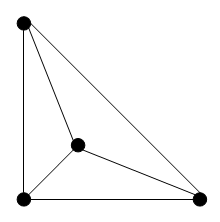
\includegraphics[width=0.33\textwidth]{figs/intro/grafo.PNG}
		\caption{Exemplo de um grafo. Fonte: Wikipedia.}
		\label{fig:grafo}
	\end{figure}
	
	Vários sistemas tomam a forma de redes, como a \emph{Web} e as Redes Sociais digitais \cite{Newman2003}. No caso do Facebook e Twitter, por exemplo, as redes são enormes, atingindo facilmente centenas de milhões de nós (usuários), levando a matrizes de dimensão equivalente a essa ordem de grandeza \cite{twitter2010}. Nesses casos, extrair informações estruturais por meio dos seus autovalores é uma tarefa desafiadora. Portanto, é necessário encontrar novos métodos com potencial para uso de computação de alto desempenho.
	
	Apresento nessa dissertação o estudo de um método com esse potencial. Em uma série de artigos, \cite{metodo2004} o primeiro, é proposta uma maneira de encontrar o autovalor mínimo de uma matriz simétrica. Para isso fazem uso de Algoritmos Genéticos, que são intrinsecamente paralelos \cite{Mitchell98,  Linden2008} e, dependendo do problema modelado e da arquitetura de computação paralela escolhida, altamente escaláveis. Essas características já foram exploradas de maneira sistemática em arquiteturas tradicionais \cite{Cantu-Paz2000}, e mais recentemente bons desempenhos foram atingidos com GAs simples executados em placas de vídeo (GPUs) com arquitetura NVIDIA CUDA. Em \cite{onemaxNaGPU} o GA paralelizado na GPU chegou a ser até trinta vezes mais rápido.

	Assim, inicialmente os principais objetivos para o projeto foram:
	
	\begin{enumerate}
		\item Desenvolver um programa serial que implementasse o método apresentado em \cite{metodo2004};
		
		\item Reproduzir os resultados de \cite{metodo2004};
		
		\item Desenvolver uma versão paralela do programa na arquitetura NVIDIA CUDA;
		
		\item Comparar o desempenho do programa Serial com o programa Paralelo.
	\end{enumerate}
	
	A \textbf{hipótese} era que o programa paralelo seria mais rápido, e o objetivo era quantificar esse ganho. Porém, a pesquisa tomou outro rumo.
	
	Encontrei uma falha em \cite{metodo2004}. O artigo afirma que o método obtém sempre o autovalor mínimo de matrizes simétricas. Com base em resultados experimentais próprios, em conhecidas propriedades do Quociente de Rayleigh e em um erro lógico no \emph{paper} em questão, argumento que não há garantias de se encontrar o menor autovalor. De fato, para a matriz de teste escolhida, \emph{em nenhuma execução} o menor autovalor foi obtido. É possível que os autores tenham omitido algum procedimento específico.
	
	Dos artigos que expõem o método \cite{metodo2004, metodo2006, metodo2008, metodo2009, metodo2011}, o último possui uma diferença significativa: a Função de Avaliação (\emph{fitness}) do Algoritmo Genético foi alterada. Essa função tem papel fundamental em todo algoritmo genético, pois é a maneira utilizada pelos GAs para determinar a qualidade de um indivíduo como solução do problema. Isso me motivou a estudar \cite{metodo2011} em detalhes, e identifiquei que, justamente por causa do novo \emph{fitness}, o erro lógico dos anteriores não foi cometido.
	
	Dado o contexto, surgiram duas hipóteses:
	
	\textbf{Hipótese 1}: a impossibilidade de se obter o menor autovalor com \cite{metodo2004} reside não em uma falha do método, mas apenas na má definição da Função de Avaliação.
	
	\textbf{Hipótese 2}: se a Hipótese 1 é verdadeira, é possível encontrar o menor autovalor com a Função de Avaliação de \cite{metodo2011}.
		
	A fim de verificar essas hipóteses, implementei um GA contendo os principais elementos comuns entre \cite{metodo2004} e \cite{metodo2011}. A ideia foi, mantendo uma única estrutura, comparar apenas o efeito da mudança do \emph{fitness}. Propus mais três funções de avaliação que, na prática, são combinações da originais.
	
	Os resultados obtidos foram satisfatórios. As duas hipóteses foram confirmadas. Para a classe de matrizes utilizadas nos testes, construí uma equação empírica para um parâmetro que aparece em todos os \emph{fitness}. O código fonte do \emph{software} utilizado está disponível na \emph{Web}. Uma versão paralelizada em GPU de um GA simples foi apresentada na III Escola Regional de Alto Desempenho de São Paulo (ERAD).